%        File: arfc-beamer.tex
%     Created: Sun May 5 10:00 PM 2013 C
%


%\documentclass[11pt,handout]{beamer}
\documentclass[9pt]{beamer}
\usetheme[white]{Illinois}
%\title[short title]{long title}
\title[Short Title]{The University of Illinois Energy Mix}
%\subtitle[short subtitle]{long subtitle}
\subtitle[Short SubTitle]{Micro-reactor Group Meeting}
%\author[short name]{long name}
\author[Your Name]{Samuel G. Dotson\\Advanced Reactors and Fuel Cycles Group}
%\date[short date]{long date}
\date[12.05.2019]{December 5, 2019}
%\institution[short name]{long name}
\institute[UIUC]{University of Illinois at Urbana-Champaign}

%\usepackage{bbding}
\usepackage{amsfonts}
\usepackage{amsmath}
\usepackage{xspace}
\usepackage{graphicx}
\usepackage{subfigure}
\usepackage{booktabs} % nice rules for tables
\usepackage{microtype} % if using PDF
\usepackage{bigints}
\usepackage{minted}
\usepackage{varwidth}
\usepackage{tabularx}
\usepackage{tikz}
\usepackage{float}
\usepackage{adjustbox}
\usepackage{caption}
\usetikzlibrary{shapes.geometric, arrows, chains}
\usetikzlibrary[calc]



%%%%%%%%%%%%%%%%%%%%%%%%%%%%%%%%%%%%%%%%%%%%%%%%%
%% Tikz commands
%%%%%%%%%%%%%%%%%%%%%%%%%%%%%%%%%%%%%%%%%%%%%%%%%
\tikzstyle{load} = [rectangle, minimum width=1cm, minimum height=1cm, text centered, draw=black, execute at begin node = \begin{varwidth}{5cm}, execute at end node=\end{varwidth}]
\tikzstyle{supply} = [diamond, minimum width=2cm, minimum height=1cm, text centered, draw=black, fill=orange!30, execute at begin node = \begin{varwidth}{1.5cm}, execute at end node=\end{varwidth}]
\tikzstyle{decision} = [circle, minimum width=1cm, minimum height=1cm, text centered, draw=black, execute at begin node = \begin{varwidth}{1.5cm}, execute at end node=\end{varwidth}]
\tikzstyle{arrow} = [thick,->,>=stealth]
\tikzstyle{extra} = [rectangle, minimum width=1cm, minimum height=1cm, text centered, draw=black, fill=green!30, execute at begin node = \begin{varwidth}{3cm}, execute at end node=\end{varwidth}]
\tikzstyle{import} = [rectangle, minimum width=1cm, minimum height=1cm, text centered, draw=black, fill=red!30, execute at begin node = \begin{varwidth}{3cm}, execute at end node=\end{varwidth}]
\tikzstyle{flexible} = [diamond, minimum width=1cm, minimum height=1cm, text centered, draw=black, fill=blue!30, execute at begin node = \begin{varwidth}{3cm}, execute at end node=\end{varwidth}]


\newcommand{\units}[1] {\:\text{#1}}%
\newcommand{\SN}{S$_N$}%{S$_\text{N}$}%{$S_N$}%
\DeclareMathOperator{\erf}{erf}
%I need some complimentary error funcitons... 
\DeclareMathOperator{\erfc}{erfc}
%Those icons in the references are terrible looking
\setbeamertemplate{bibliography item}[text]

%%%% Acronym support

\usepackage[acronym,toc]{glossaries}
\include{acros}

\makeglossaries

%try to get rid of header on title page\dots
\makeatletter
    \newenvironment{withoutheadline}{
        \setbeamertemplate{headline}[default]
        \def\beamer@entrycode{\vspace*{-\headheight}}
    }{}
\makeatother

\makeatother
\setbeamertemplate{footline}
{
  \leavevmode%
  \hbox{%
    \rightline{\insertframenumber{} / \inserttotalframenumber\hspace*{1ex}}
  }%
  \vskip0pt%
}
\makeatletter
\begin{document}
%%%%%%%%%%%%%%%%%%%%%%%%%%%%%%%%%%%%%%%%%%%%%%%%%%%%%%%%%%%%%
%% From uw-beamer Here's a handy bit of code to place at 
%% the beginning of your presentation (after \begin{document}):
\newcommand*{\alphabet}{ABCDEFGHIJKLMNOPQRSTUVWXYZabcdefghijklmnopqrstuvwxyz}
\newlength{\highlightheight}
\newlength{\highlightdepth}
\newlength{\highlightmargin}
\setlength{\highlightmargin}{2pt}
\settoheight{\highlightheight}{\alphabet}
\settodepth{\highlightdepth}{\alphabet}
\addtolength{\highlightheight}{\highlightmargin}
\addtolength{\highlightdepth}{\highlightmargin}
\addtolength{\highlightheight}{\highlightdepth}
\newcommand*{\Highlight}{\rlap{\textcolor{HighlightBackground}{\rule[-\highlightdepth]{\linewidth}{\highlightheight}}}}
%%%%%%%%%%%%%%%%%%%%%%%%%%%%%%%%%%%%%%%%%%%%%%%%%%%%%%%%%%%%%
%%--------------------------------%%
\begin{withoutheadline}
\frame{
  \titlepage
}
\end{withoutheadline}

%%--------------------------------%%
\AtBeginSection[]{
\begin{frame}
  \frametitle{Outline}
  \tableofcontents[currentsection]
\end{frame}
}

\section{Overview}
% \subsection{Overview}
\begin{frame}
  \frametitle{Overview}
  % a comment
  \begin{adjustbox}{max totalsize={0.9\textwidth}{0.7\textheight}, center}
    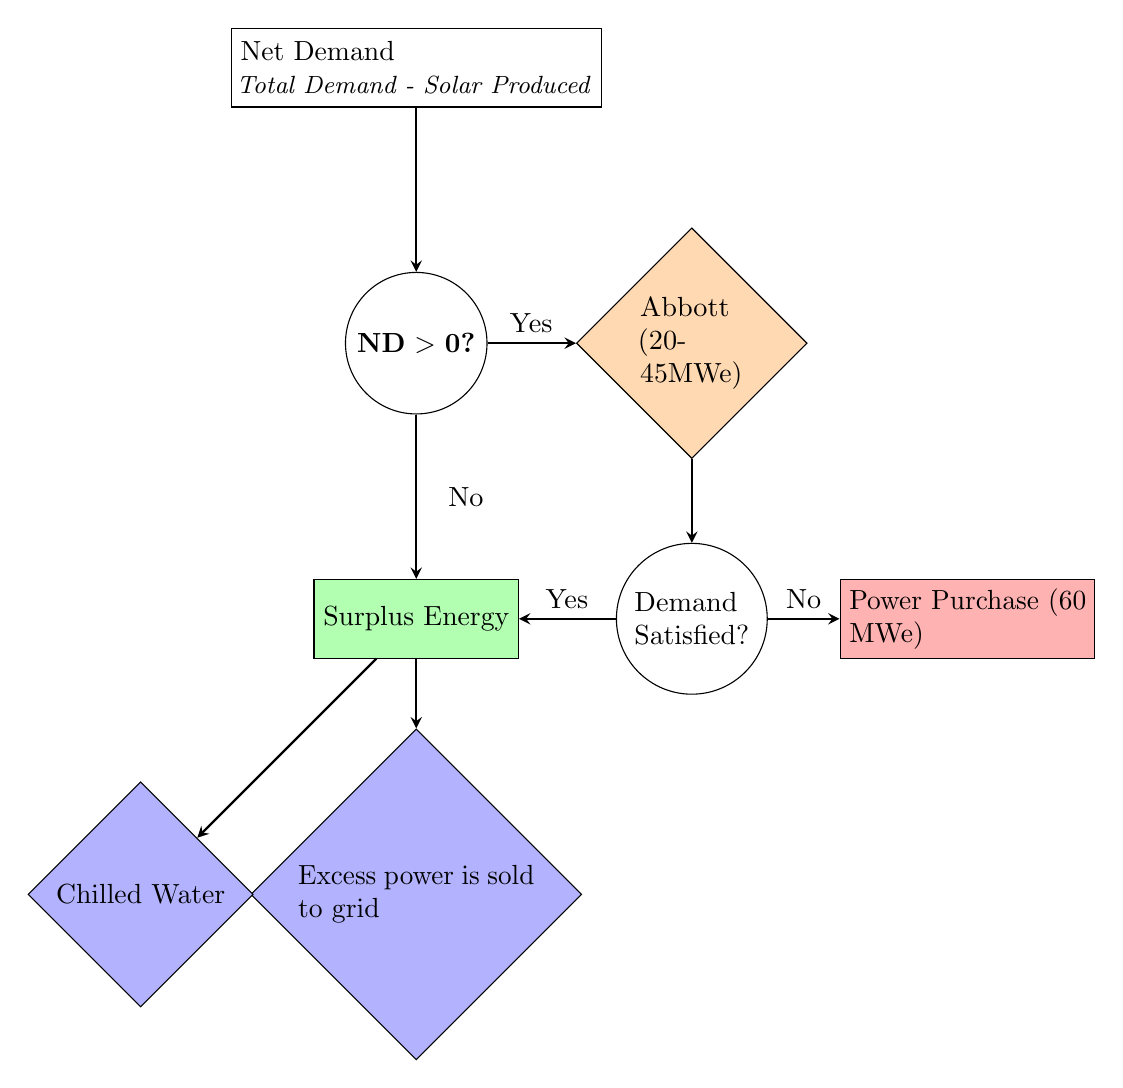
\begin{tikzpicture}[node distance = 3.5cm, auto, scale=0.25]
        \node (demand) [load] {Net Demand\\\small{\textit{Total Demand - Solar Produced}}};
        \node (ND) [decision, below of = demand] {\textbf{ND $>$ 0?}};
        \node (abbott) [supply, right of = ND] {Abbott (20-45MWe)};
        \node (isfull) [decision, below of = abbott] {Demand Satisfied?};
        \node (surplus) [extra, left of = isfull] {Surplus Energy};
        \node (purchase) [import, right of = isfull] {Power Purchase (60 MWe)};
        \node (buyback) [flexible, below of = surplus] {Excess power is sold to grid};
        \node (chilledwater) [flexible, left of = buyback] {Chilled Water};
  
        % \node (d1) [load, draw=none, below of = purchase] {\textbf{??}};
  
        \draw [arrow] (demand) -- (ND);
        \draw [arrow] (ND) -- node [text width = 1cm, midway, align=center] {No} (surplus);
        \draw [arrow] (ND) -- node [text width = 1cm, midway, above, align=center] {Yes} (abbott);
        \draw [arrow] (abbott) -- (isfull);
        \draw [arrow] (isfull) -- node [text width = 1cm, midway, above, align=center] {Yes} (surplus);
        \draw [arrow] (isfull) -- node [text width = 2cm, midway, above, align=center] { No } (purchase);
        \draw [arrow] (surplus) -- (chilledwater);
        % \draw [arrow] (purchase) -- (d1);
        \draw [arrow] (surplus) -- (buyback);
      \end{tikzpicture}
    
  \end{adjustbox}

  \captionof{figure}{The University of Illinois Energy Prioritization}

  \end{frame}
  % }

% \subsection{Abbott}
\section{Campus Energy Needs}
\subsection{Electricity}
\begin{frame}

	\begin{figure}
		\centering
		\includegraphics[width=0.9\textwidth]{./images/typical_demand.png}
		\caption*{The typical yearly electricity demand for UIUC. Average need is about 45 MWe, peaks near 80MWe.}
	\end{figure}

\end{frame}
\subsection{Steam}
\begin{frame}

	\begin{figure}
		\centering
		\includegraphics[width=0.9\textwidth]{./images/typical_steam.png}
		\caption*{The typical yearly steam demand for UIUC. Typical need is about 150 klbs/hr, peaks in the winter over 300klbs/hr.}
	\end{figure}

	
\end{frame}
\section{Systems}
\subsection{Abbott}
    \begin{frame}
  \frametitle{Abbott Power Plant}
  % a comment
        \begin{columns}
                \column[t]{5cm}
                Quick Facts \cite{noauthor_abbott_nodate}
                \begin{enumerate}
                    \item Cogeneration Plant (electricity is a ``byproduct'' of steam production).
                    \item Capable of producing 85 MWe (maximum capacity).
                    \item Capable of producing 800 Klbs/hr of steam (maximum capacity).
                \end{enumerate}
                \column[t]{5cm}
        \begin{figure}[htbp!]
        \begin{center}
      \includegraphics[height=4cm]{./images/abbott.jpg}
    \end{center}
          \caption*{South side of Abbott Power Plant.}
    \label{fig:abbott}
  \end{figure}
        \end{columns}
\end{frame}



\subsection{Solar Farm}
\begin{frame}
	
\begin{columns}
	\column[t]{5cm}
	Quick Facts \cite{white_solar_2017}
	\begin{itemize}
		\item Lifetime capacity factor of 16.8\%. 
		\item Rated to produce 4.8 MWe
		\item Soon to be expanded to 12.1 MWe
	\end{itemize}
	\column[t]{5cm}
	\begin{figure}
		\centering
		\label{fig:solarfarm}
		\includegraphics[width=0.8\textwidth]{./images/solarfarm.jpeg}
		\caption*{UIUC Solar Farm}
	\end{figure}
\end{columns}
	\begin{figure}
		\centering
		\label{fig:solardata}
		\includegraphics[width=0.75\textwidth]{./images/actual_solarfarm_9-1-2016.png}
		\caption{Actual solar farm data from AlsoEnergy \cite{alsoenergy_university_2019}}
	\end{figure}
\end{frame}

\begin{frame}
	\begin{figure}
		\centering
		\label{fig:typical_solar}
		\includegraphics[width=0.9\textwidth]{./images/typical_solarpower.png}
		\caption{The typical power output of the UIUC solarfarm over a year.}
	\end{figure}
\end{frame}
\subsection{Power Purchase Agreement}
\begin{frame}
\Large{Power Purchase Agreements}\\


Quick Facts \cite{breitweiser_wind_2016}:

\begin{itemize}
	\item Power purchase agreement (PPA) with Rail Splitter Wind Farm
	\item PPA requires UIUC to buy 8.6\% of the energy produced by the wind farm.
	\item Fixed price of 4 cents/KWh
	\item Sometimes sold back at loss.\\
	e.g. A windy night when demand is low but the wind farm is producing a lot of electricity.
\end{itemize}
	
\end{frame}
\subsection{Chilled Water}
\begin{frame}

	\Large{Chilled Water}\\

	Quick facts \cite{noauthor_campus_nodate}:
	\begin{itemize}
		\item The energy consumption from chilled water is felt as electricity* demand.
		\item The only method of energy storage on campus. 
	\end{itemize}

	\small{*There are also steam driven chillers that are not currently being used.}
\end{frame}
\section{Current Work}
\begin{frame}
	\large Current Work\\

	\begin{itemize}
		\item Finding the optimal size of a reactor to minimize the cost of electricity and steam. \\
		Based on a paper \cite{baker_optimal_2018} that sized a reactor for a similar grid system. 
		\item F \& S intends to retire the coal boilers by 2025 and replace it with more PPAs and natural gas \cite{affiliated_engineers_inc_utilities_2015} according to the UIUC Energy Master Plan, in lieu of alternatives from ``developing technologies.'' These decisions were made to minimize the cost of electricity.
	\end{itemize}

	\begin{figure}
		\centering
		\label{fig:masterplan}
		\includegraphics[width=0.75\textwidth]{./images/masterplan.png}
		\caption{Current trajectory \cite{affiliated_engineers_inc_utilities_2015}}
	\end{figure}
\end{frame}
% \input{acks}
%%--------------------------------%%
%%--------------------------------%%
\begin{frame}[allowframebreaks]
  \frametitle{References}
  \bibliographystyle{plain}
  {\footnotesize \bibliography{bibliography.bib} }

\end{frame}

%%--------------------------------%%


\end{document}



